\section{Results}

Hereafter we list the messages peers exchange in Multipong and their
size\footnote{the size shown in the table has to be intended as ``greater or
equal than''}:

\begin{table}[H]
  \centering
  \begin{tabular}{l|c c}
  & \textbf{\textit{Message}} & \textbf{\textit{Size [B]}}  \tabularnewline
            \hline
            \multirow{5}{*}{TCP} & \multicolumn{1}{c}{\texttt{ARE\_YOU\_HOST}} & \multicolumn{1}{c}{60} \\\cline{2-3}
                                 & \multicolumn{1}{c}{\texttt{AVAILABLE}} & \multicolumn{1}{c}{100} \\\cline{2-3}
                                 & \multicolumn{1}{c}{\texttt{CANCEL}} & \multicolumn{1}{c}{56} \\\cline{2-3}
                                 & \multicolumn{1}{c}{\texttt{DISCOVERY}} & \multicolumn{1}{c}{82} \\\cline{2-3}
                                 & \multicolumn{1}{c}{\texttt{JOIN}} & \multicolumn{1}{c}{54} \\\hline
            \multirow{3}{*}{UDP} & \multicolumn{1}{c}{\texttt{KNOWN\_HOSTS}} & \multicolumn{1}{c}{90} \\\cline{2-3}
                                 & \multicolumn{1}{c}{\texttt{STARTING}} & \multicolumn{1}{c}{187} \\\cline{2-3}
                                 & \multicolumn{1}{c}{\texttt{TELL\_IP}} & \multicolumn{1}{c}{57} \\\hline
        \end{tabular}
  \caption{Messages size}
  \label{tab:sizes}
\end{table}

The average power consumption and Wi-Fi Direct traffic can be seen in Figure
\ref{fig:comparison}.

\begin{figure}[H]
  \centering
  \begin{tabular}{@{}c@{}c}
      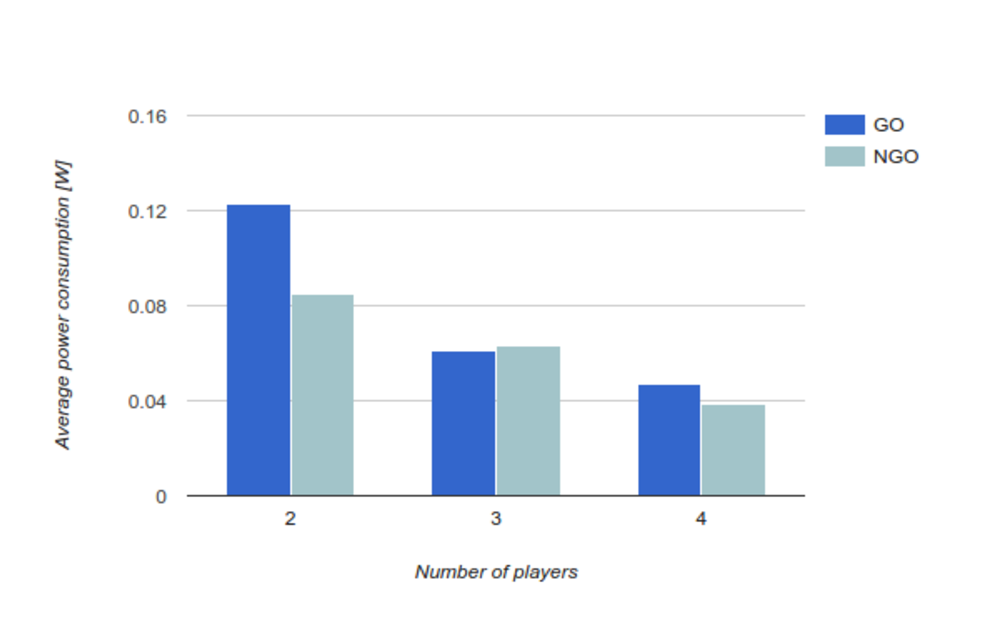
\includegraphics[width=.5\columnwidth]{img/energy.eps}
      \label{fig:energy}
    &
    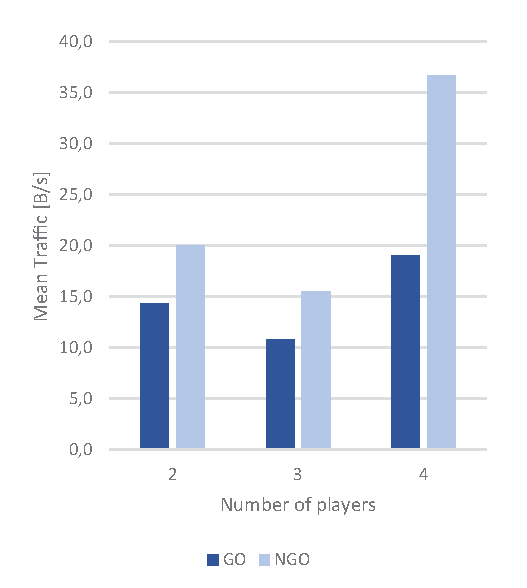
\includegraphics[width=.5\columnwidth]{img/traffic.eps}
    %\caption{Energy consumption comparison}
    \label{fig:traffic}
  \end{tabular}
  \caption{GO/NGO comparison for energy and traffic}\label{fig:comparison}
\end{figure}

% TODO: Network traffic --
% TODO: 2 - 4 players comparison
% TODO: Explain why sometimes NGO > GO

% TODO: Power consumption is too variable: PowerTutor, network instability,
%       touching the screen impacts on power consumption
